\chapter{HW implementering og test}

\section{Implementering}

\subsection{Forstærkerblok}
Som forstærkerblok anvendes INA114, se Figur 3.1. Denne har den fordel, at gain kan kontrolleres af en variabel modstand (potentiometer), $R_{G}$. 

\begin{figure}[H]
	\centering
	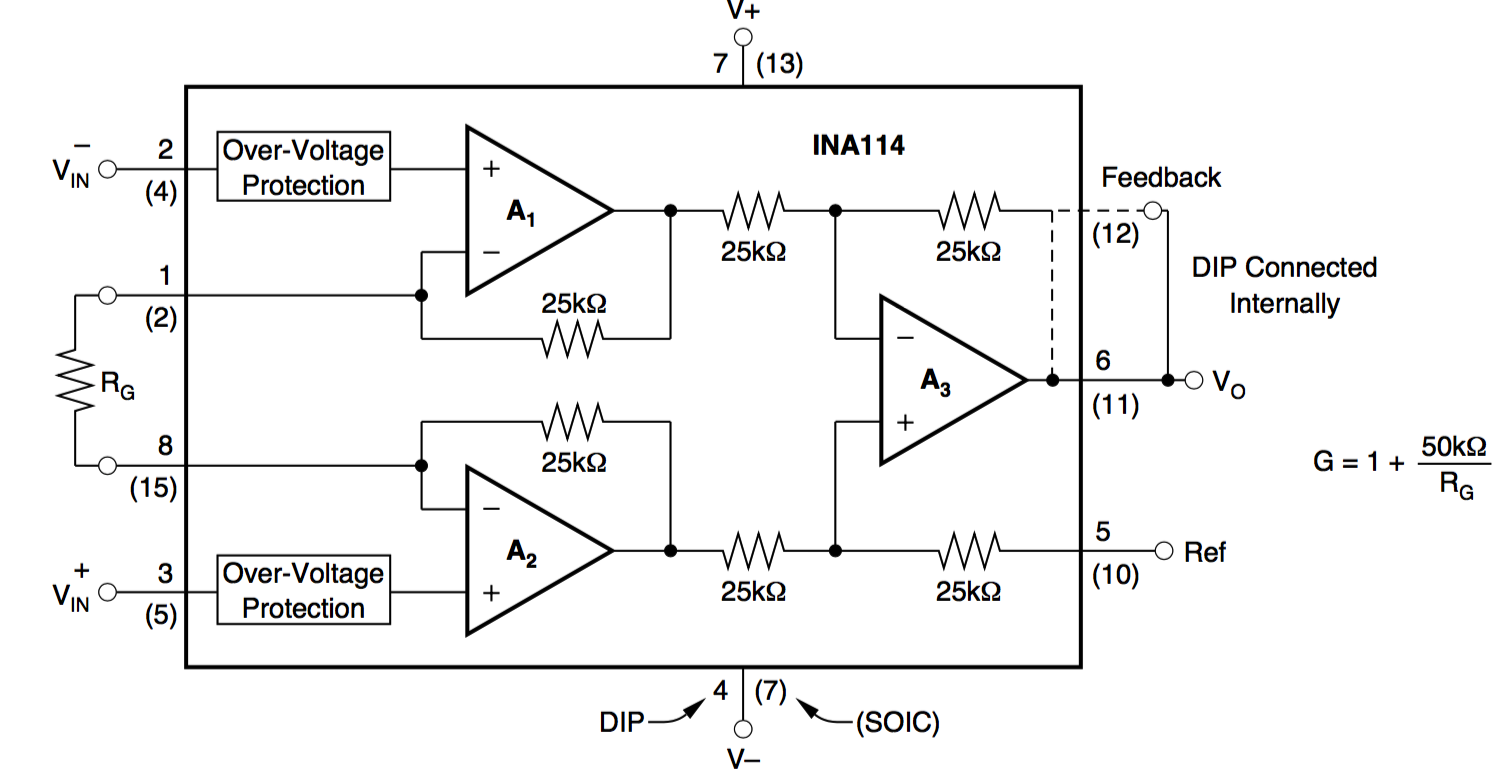
\includegraphics[width=1\textwidth]{Figurer/Snip20151117_104}
	\caption{INA114}
\end{figure}

INA114 er blevet udleveret som én komponent. Den sorte boks på Figur 3.1 viser, hvilke komponenter INA114 indeholder. Det ses også, at $R_{G}$ er placeret udenfor den sorte boks, hvilket betyder, at det er en variabel modstand, der skal tilkobles INA114.     

\subsubsection{Forstærkning}
Forstærkningen, Gain, skal forstærke den maksimale inputsspænding fra tryktransduceren, så outputtet bliver 5 V, hvilket er det maksimale DAQ'en kan registrere. Udregningen for forstærkning kan ses i ligning (2.4) til (2.5).
\begin{equation}
	Gain = 370
\end{equation}


\subsubsection{Båndbredde}
For INA114 er produktet af båndbredden og forstærkningen en konstant på 1.000.000 \footnote{Se datablad for INA114 s. 2 i bilag}.
Båndbredden for denne forstærkerblok, hvor gain er 370, er 

\begin{equation}
	Gain \cdot BW = 1.000.000 \\ \Longrightarrow \\
	BW = \frac{1.000.000}{370} \\ \Longrightarrow \\
	BW = 2702 Hz
\end{equation} 

Båndbredden er større end 50 Hz, som var det, båndbredden mindst skulle være. 

\subsubsection{Gainmodstand}
Gainmodstanden, $R_{G}$ er en variabel modstand, der bestemmer forstærkningen i INA114. INA114 skal have en gain på 370. Ud fra ligning (3.3) kan $R_{G}$ isoleres og beregnes.\\

\begin{equation}
	Gain = 1+\frac{50k\Omega}{R_g} \\ \Longrightarrow \\
	R_{G} = \frac{50k\Omega}{Gain - 1} \\ \Longrightarrow \\
	R_{G} = \frac{50k\Omega}{370 - 1} \\ \Longrightarrow \\
	R_{G} = 135,5\Omega
\end{equation}


\section{Filterblok}
Som filter anvendes et Sallen Key lavpasfilter med unity gain.

\begin{figure}[H]
	\centering
	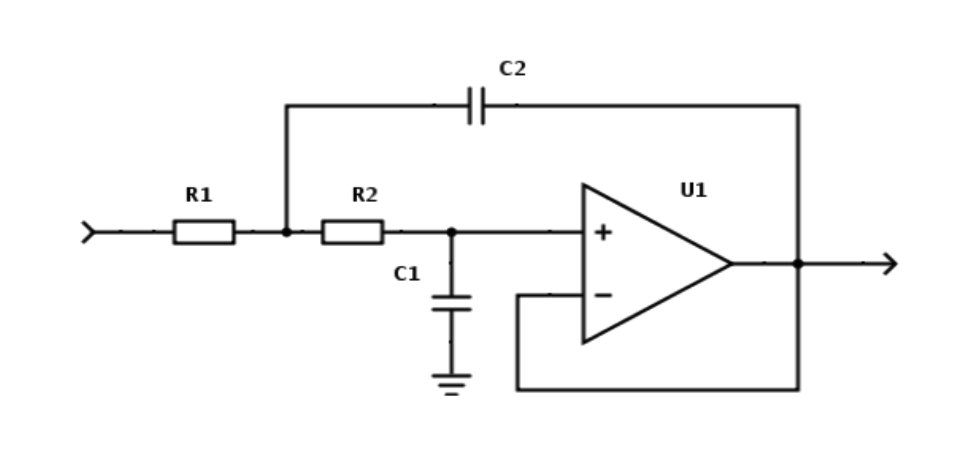
\includegraphics[width=1\textwidth]{Figurer/Snip20151117_105}
	\caption{Sallen Key lavpasfilter}
\end{figure}

\subsection{Beregning af komponentværdier}
Ud fra overføringsfunktion for filteret kan de forskellige komponentværdier beregnes. 

\subsubsection{Overføringsfunktion}
\begin{align}
	\frac{V_{out}(s)}{V_{in}(s)}=\frac{\frac{1}{R_1R_2C_1C_2}}{s^2+\frac{R_1+R_2}{R_1R_2C_2}+\frac{1}{R_1R_2C_1C_2}}
\end{align}

\subsubsection{Standardform}
\begin{align}
	\frac{V_{out}(s)}{V_{in}(s)}=\frac{w_n^2}{s^2+2\zeta\omega _n+w_n^2}
\end{align}

\begin{align}
	\omega _n = \sqrt{\frac{1}{R_1R_2C_1C_2}}
\end{align}

Kondensatoren, C2, skal være 680 nF og kondensatoren, C1, bestemmes til 340 nF, da denne kondensator kunne realiseres ud fra det, der var til rådighed. Der benyttes en kondensator på 330 nF og 10 nF til den realisering. Modstandene R1 og R2 skal være samme værdi, R = R1 = R2    

\begin{equation}
	50*2\pi = \sqrt{\frac{1}{R*340*10^{-9}*680*10^{-9}}} \\ \Longrightarrow \\
	Solve, R \\ \Longrightarrow \\
	R = 6620 \Omega
\end{equation}

\subsubsection{Magnitude Bodeplot}
Bodeplottet i Figur 3.3 viser, at ved -3 dB, hvor cutofffrekvens befinder sig er frekvensen 50 Hz, som var et krav. Det ses også, at grafen er faldet med 40 dB en dekade efter, 500 Hz, som også var et krav.   
\begin{figure}[H]
	\centering
	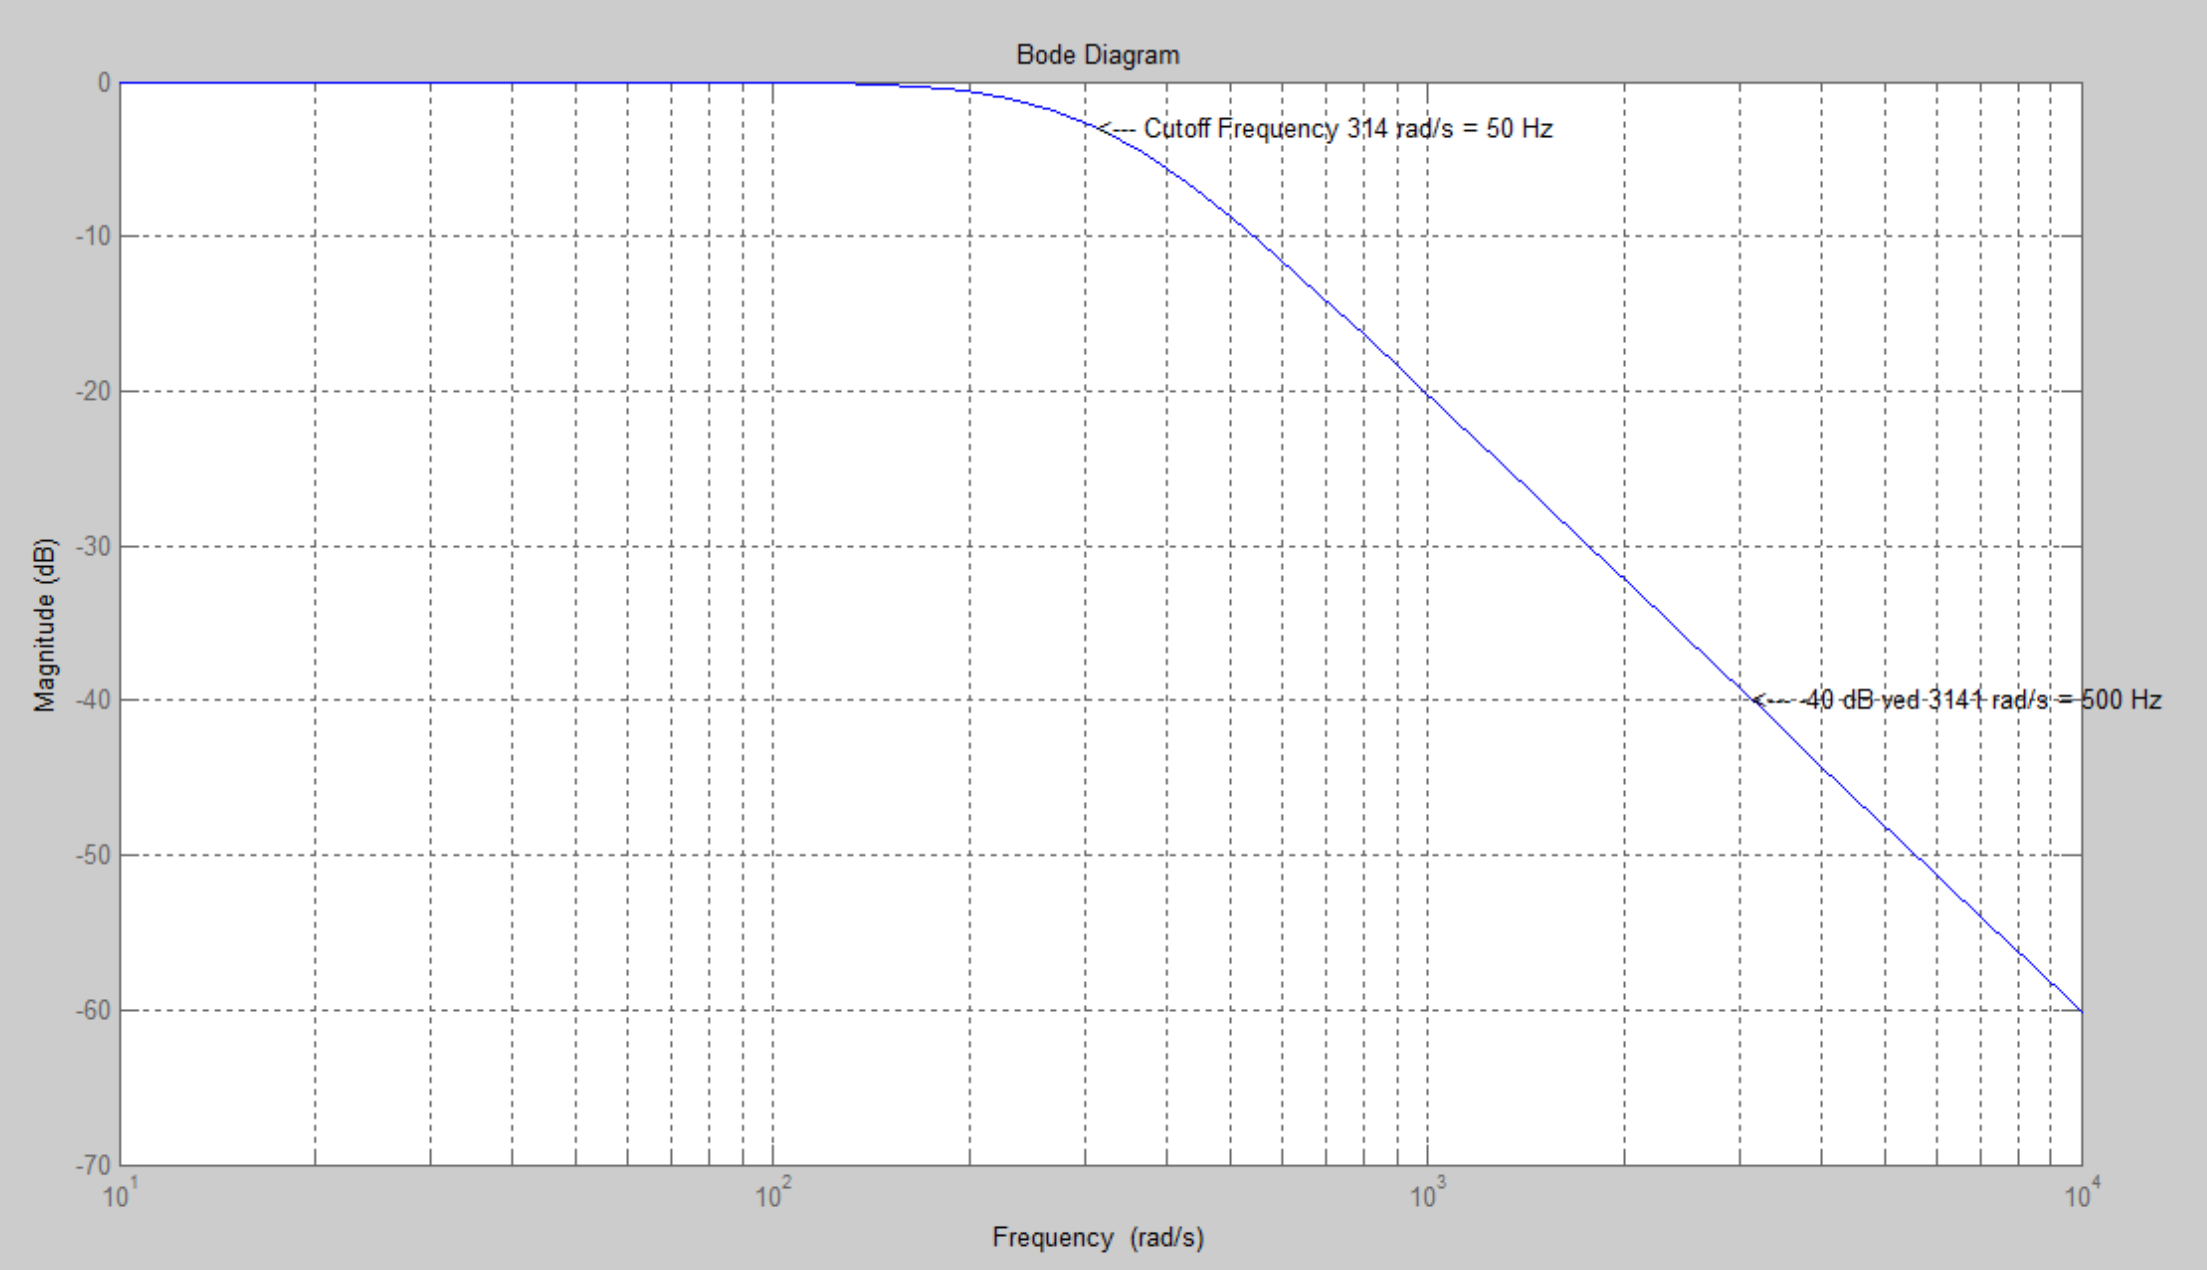
\includegraphics[width=1\textwidth]{Figurer/Bodeplot_Lavpasfilter_Teoretisk}
	\caption{Magnitude Bodeplot Lavpasfilter}
	\label{fig:Bodeplot}
\end{figure}

\section{Test}
Forstærkeren og filteret testes via Analog Discovery \& Waveforms.

\subsection{Forstærkerblok}
Testopstillingen kan ses på Figur 3.4. 

\begin{figure}[H]
	\centering
	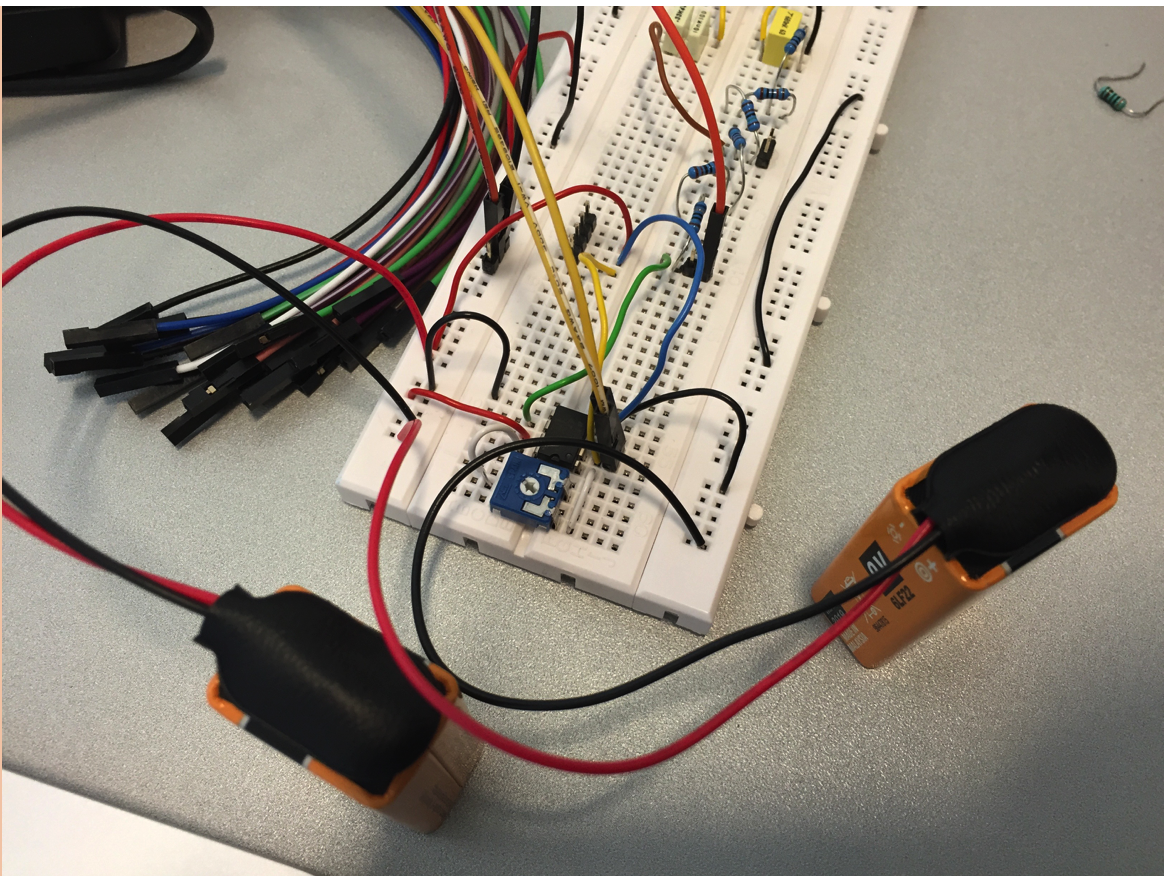
\includegraphics[width=1\textwidth]{Figurer/Snip20151117_106}
	\caption{Testopstilling for forstærkeren}
\end{figure}

Der ønskes, at ved en indgangsspænding på 13,5 mV vil outputsspændingen være forstærket op til 5 V. Der kunne ikke påtrykkes en spænding på 13,5 mV, men istedet med 13 mV. Outputsspændingen ved 13 mV er 

\begin{equation}
	13 mV \cdot 370 = 4,8 V
\end{equation} 

Dette ser, at være det samme, når man tester forstærkeren. 




\subsection{Filterblok}

Følgende målinger er udført med komponentværdier, som i praksis gav bedre resultater end komponentværdierne udregnet i teori-afsnittet. Følgende komponenter er benyttet: 
R1 og R2: 2,3, C1: 340nF og C2: 680nF. 

Målingerne er foretaget ved at påsætte filteret en AC spænding på 5V med varierende frekvens i et spekter fra 1 Hz til 500 Hz. Dette gøres for at teste frekvensresponset på filteret. 

Channel 1 er indgangsspændingen og viser den varierende frekvens. Ændringen ses i venstre side af efterfølgende skærmbilleder. 
Oscilloskopet måler udgangsspændingen på filteret og resultatet vises i højre side af efterfølgende skærmbilleder. 

Følgende målinger er udført med komponentværdier, som i praksis gav bedre resultater end komponentværdierne udregnet i teori-afsnittet. Følgende komponenter er benyttet: 
R1 og R2: 2,3, C1: 340nF og C2: 680nF. 

Målingerne er foretaget ved at påsætte filteret en AC spænding på 5V med varierende frekvens i et spekter fra 1 Hz til 500 Hz. Dette gøres for at teste frekvensresponset på filteret. 

Channel 1 er indgangsspændingen og viser den varierende frekvens. Ændringen ses i venstre side af efterfølgende skærmbilleder. 
Oscilloskopet måler udgangsspændingen på filteret og resultatet vises i højre side af efterfølgende skærmbilleder. \\
Værdierne der gerne vil opnår er henholdsvis:


\begin{longtabu} to \linewidth{@{}l X[j]@{}}
	\textbf{Input} & \textbf{Output} \\[-1ex]
	\midrule
	5V 1Hz & 5V \\[-1ex]
	5V 50Hz	& 3.53V\\[-1ex]
	5V 500Hz & 0.5 V \\[-1ex]
	\caption{}	
\end{longtabu}

	

\begin{figure}[H]
	\centering
	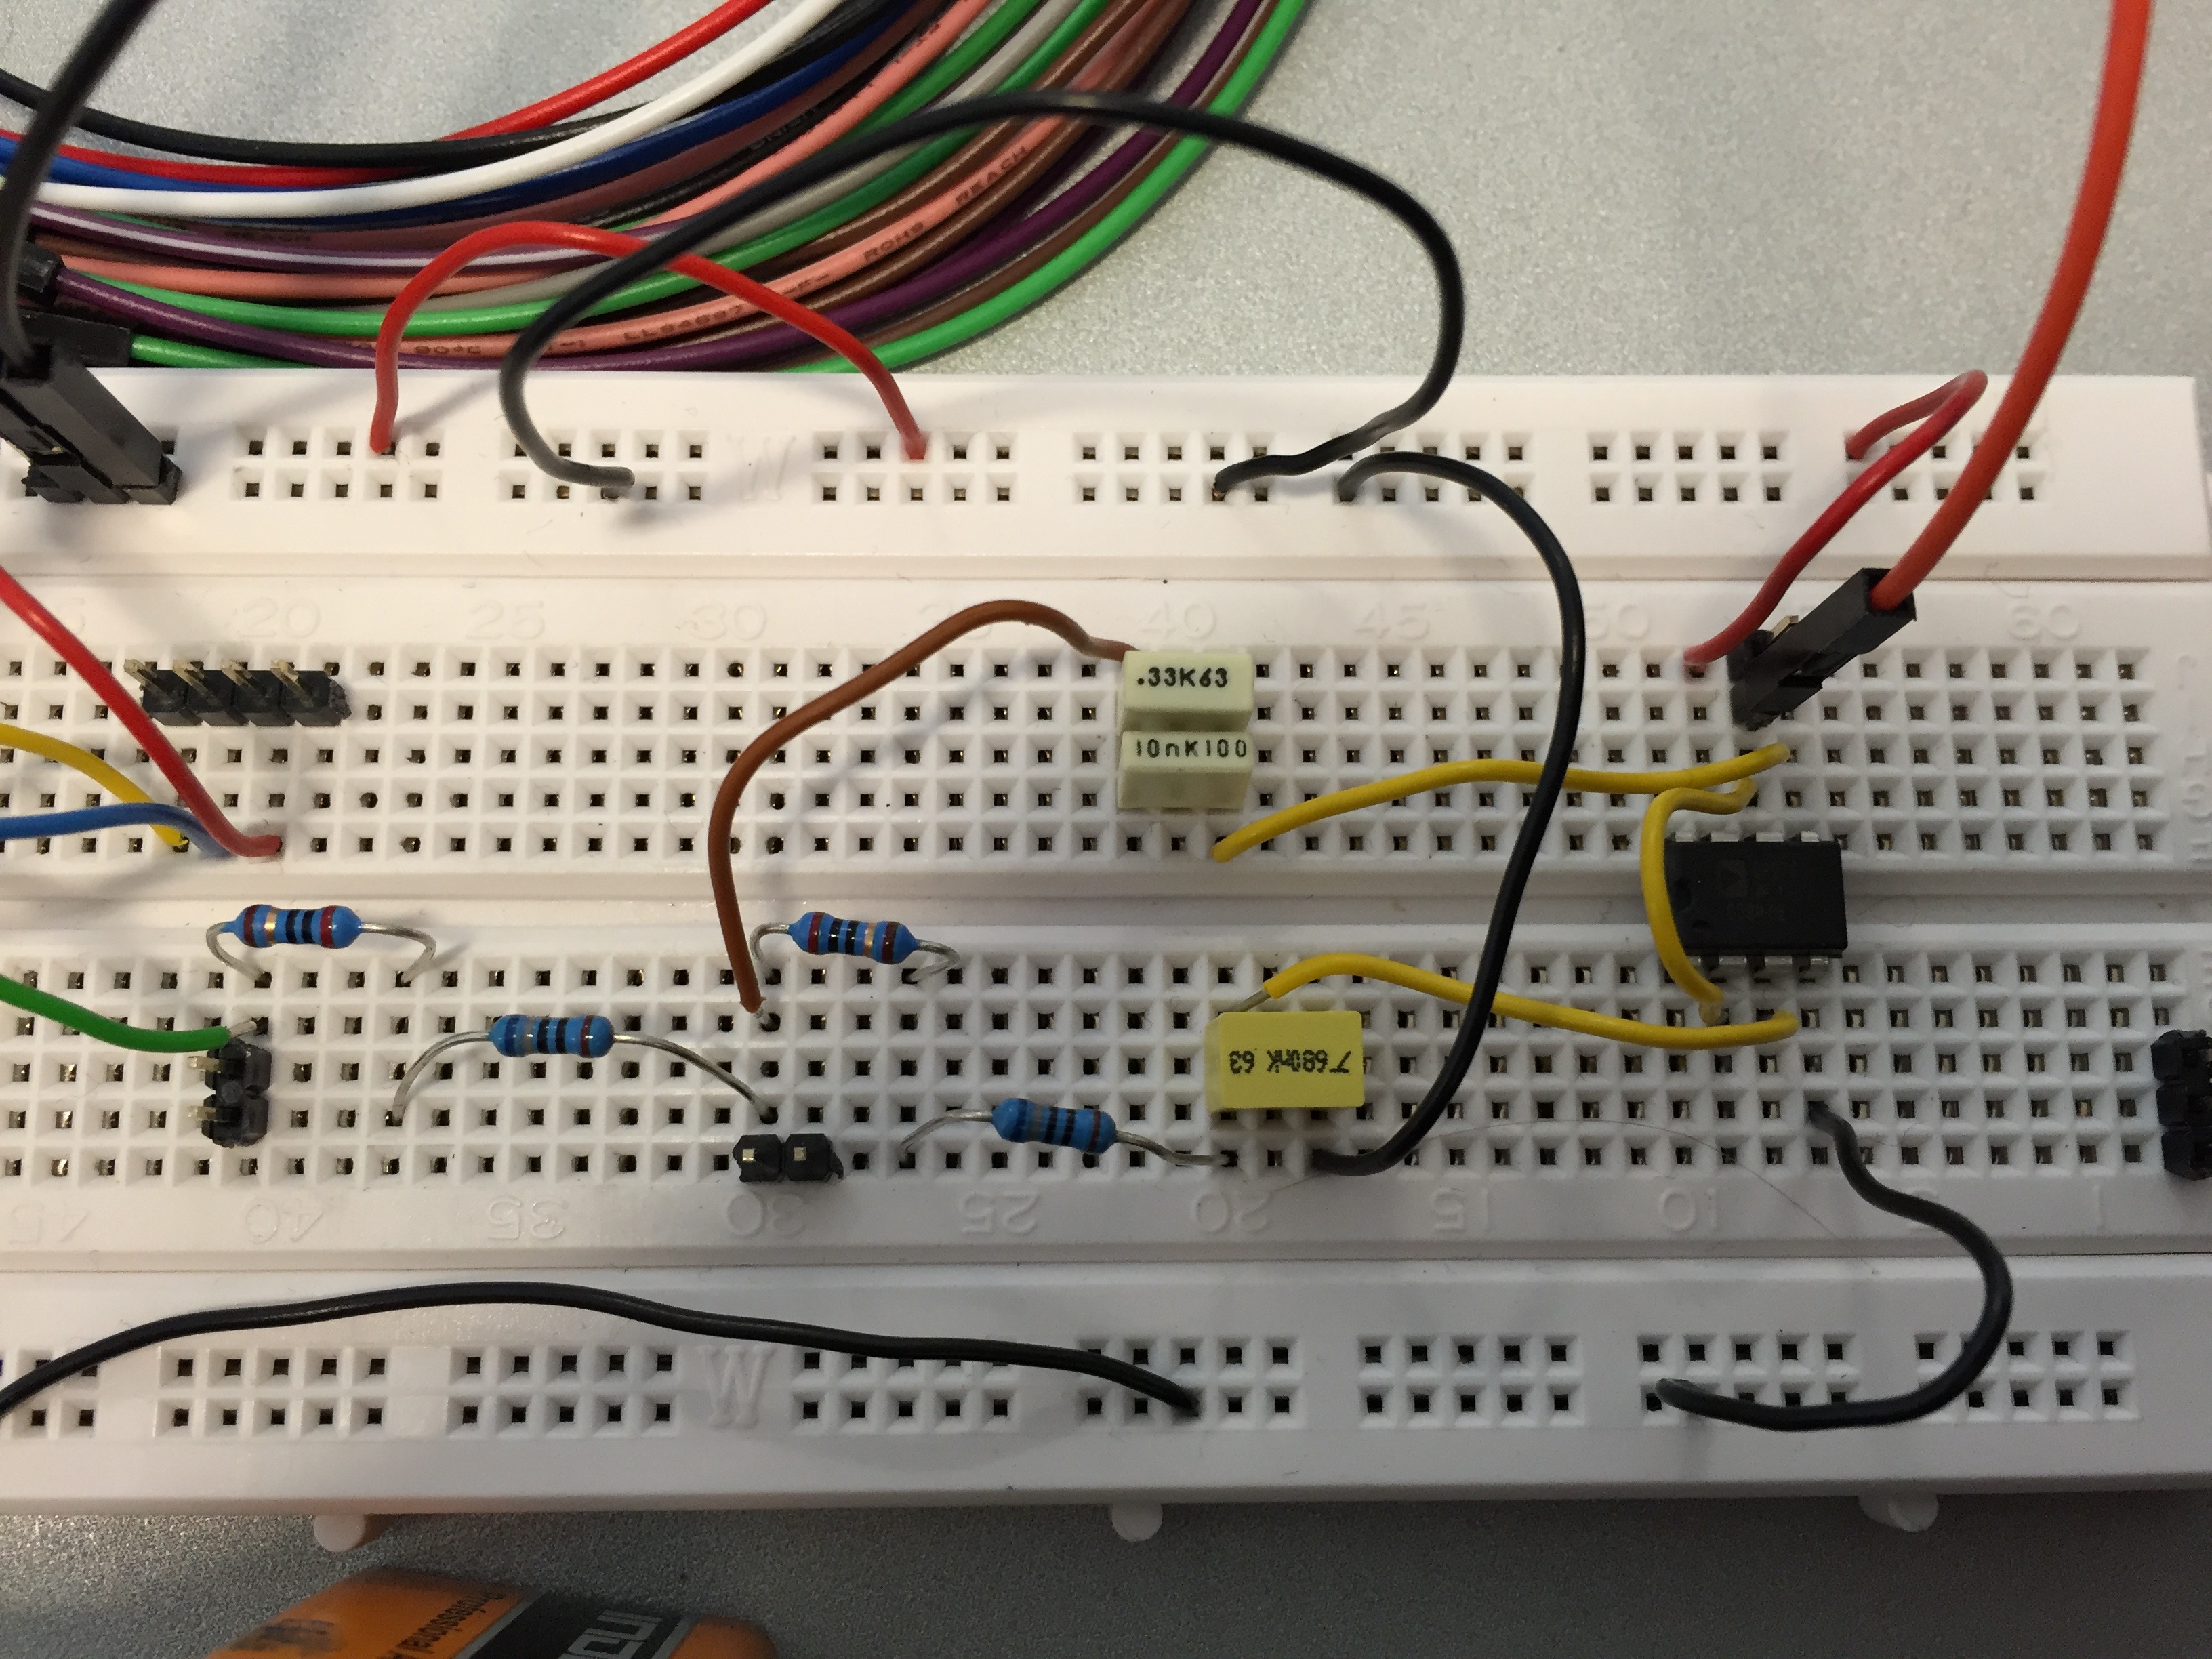
\includegraphics[width=1\textwidth]{Figurer/Filterblok}
	\caption{Praktisk opstilling af Filter}
	\label{fig:Filter}
\end{figure}

\begin{figure}[H]
	\centering
	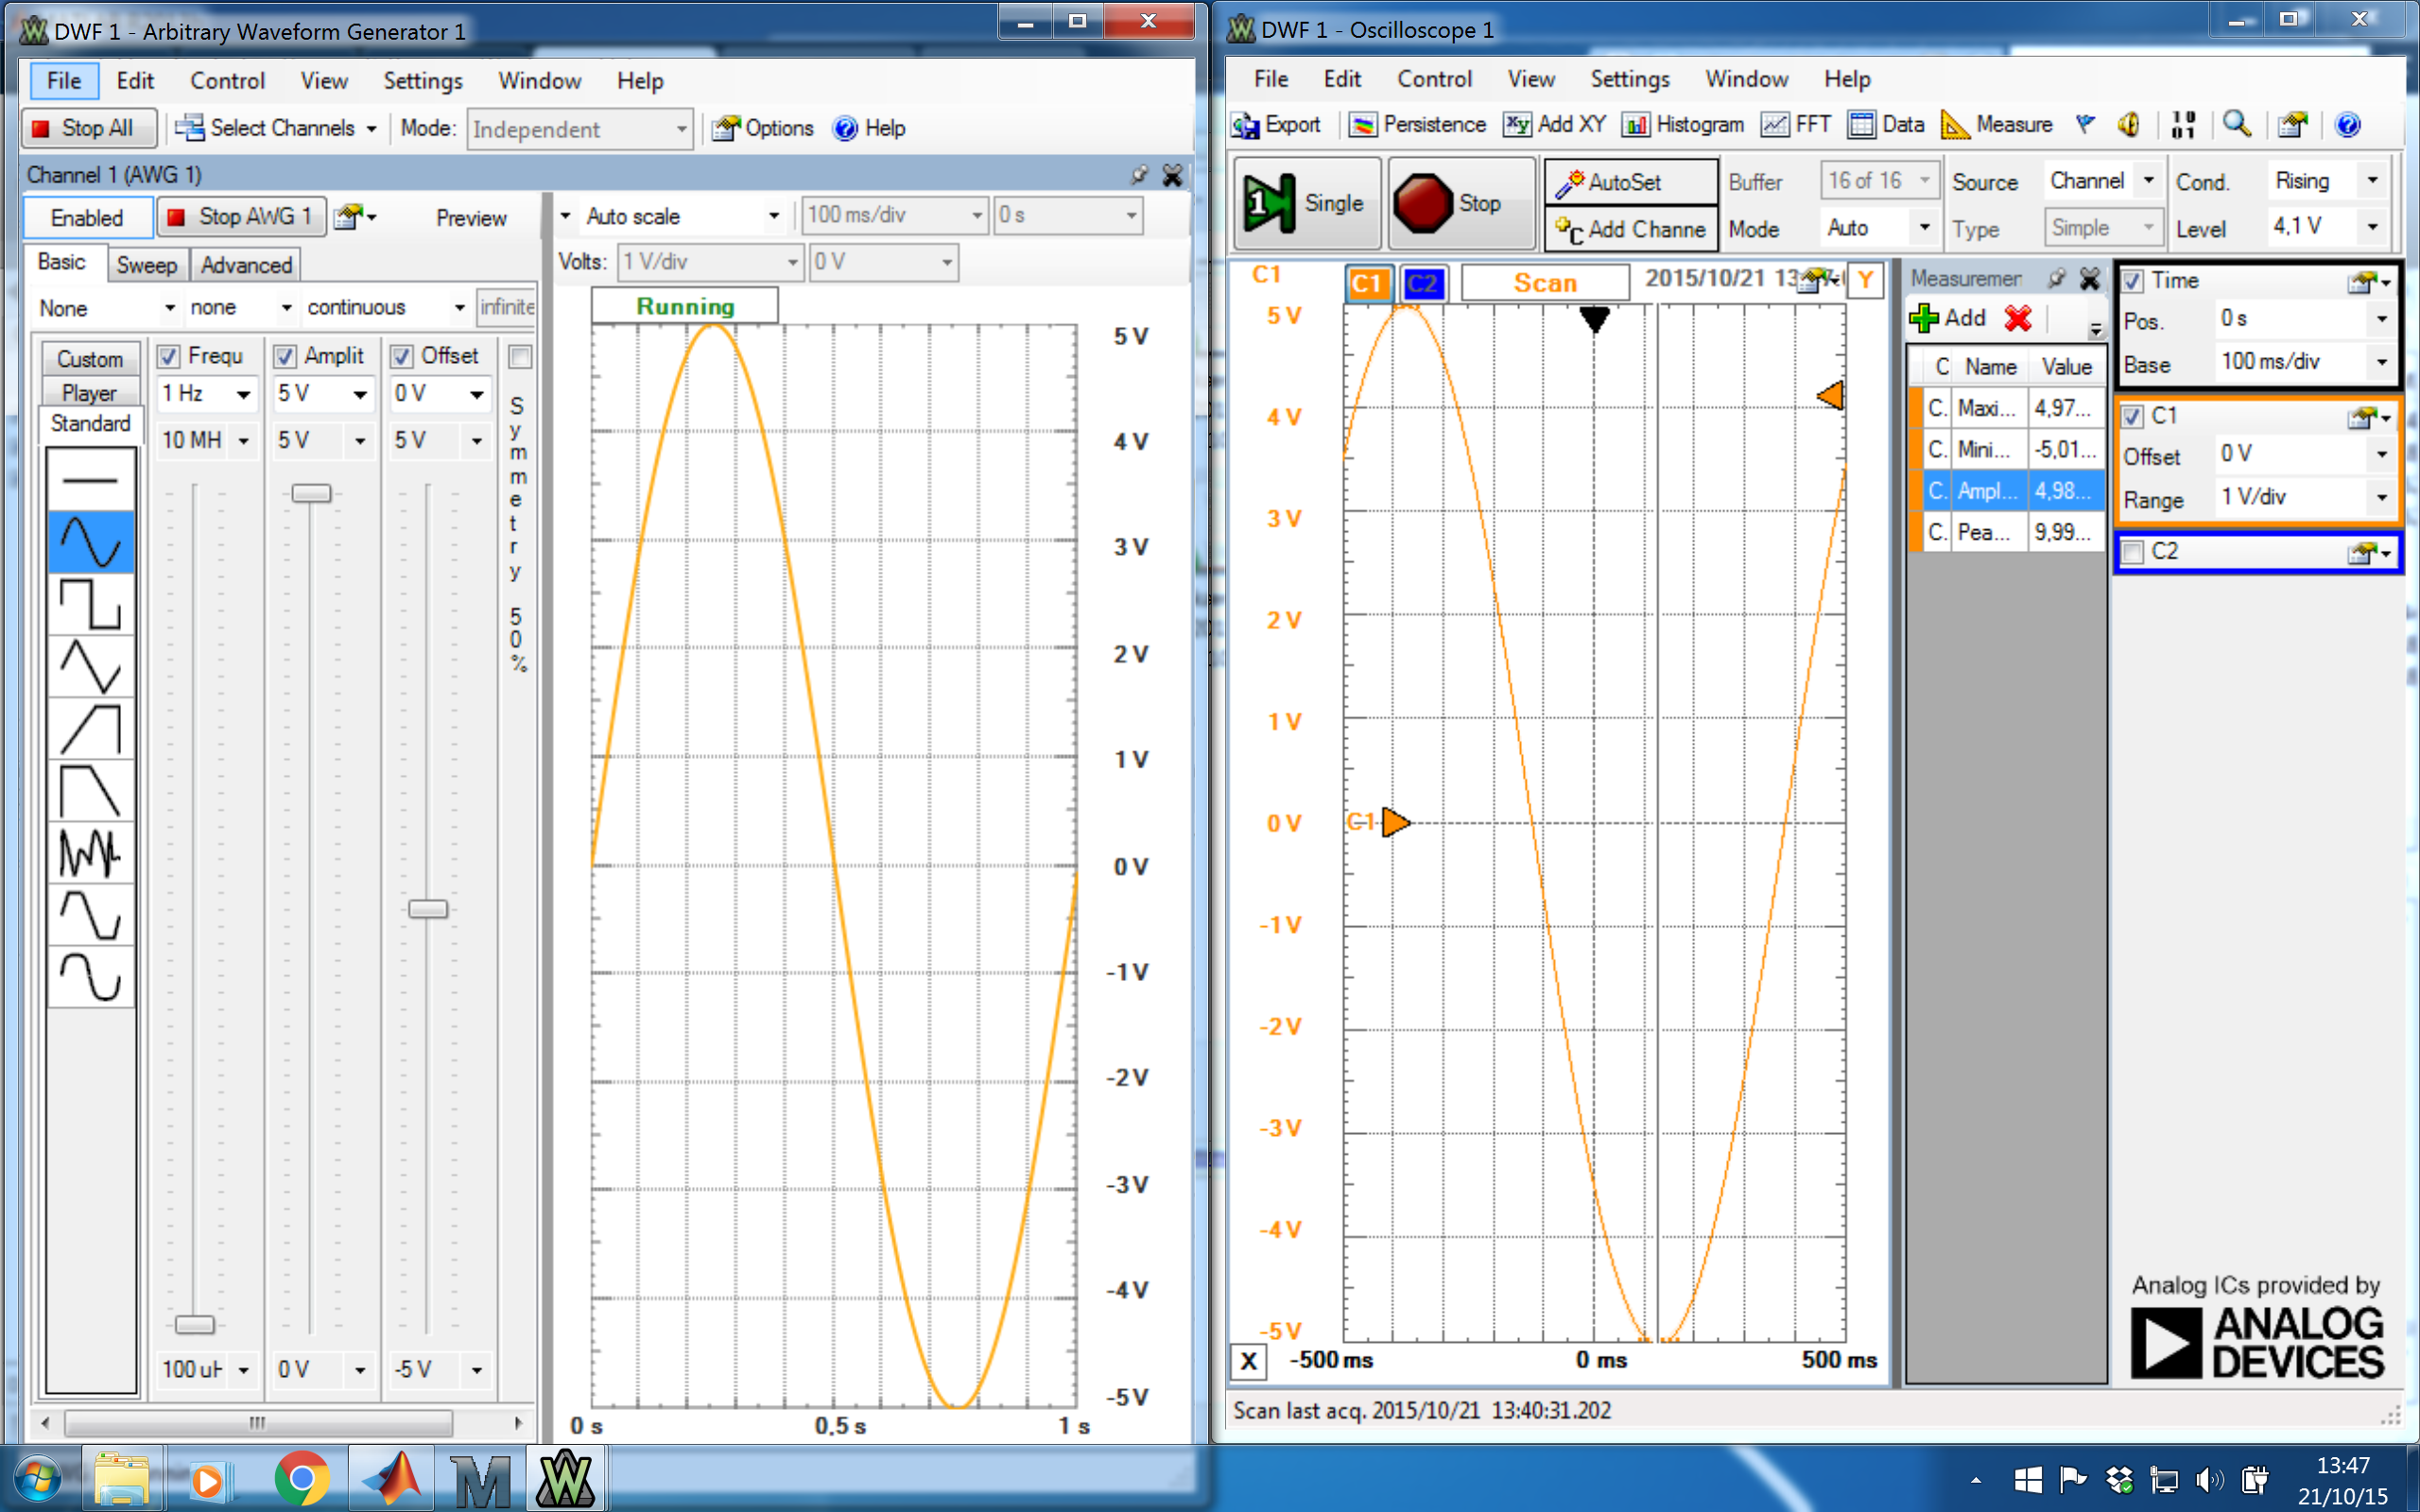
\includegraphics[width=1\textwidth]{Figurer/Lavpasfilter_Praktisk_1Hz}
	\caption{Lavpasfilter respons 1 Hz}
	\label{fig:Filter}
\end{figure}

\begin{figure}[H]
	\centering
	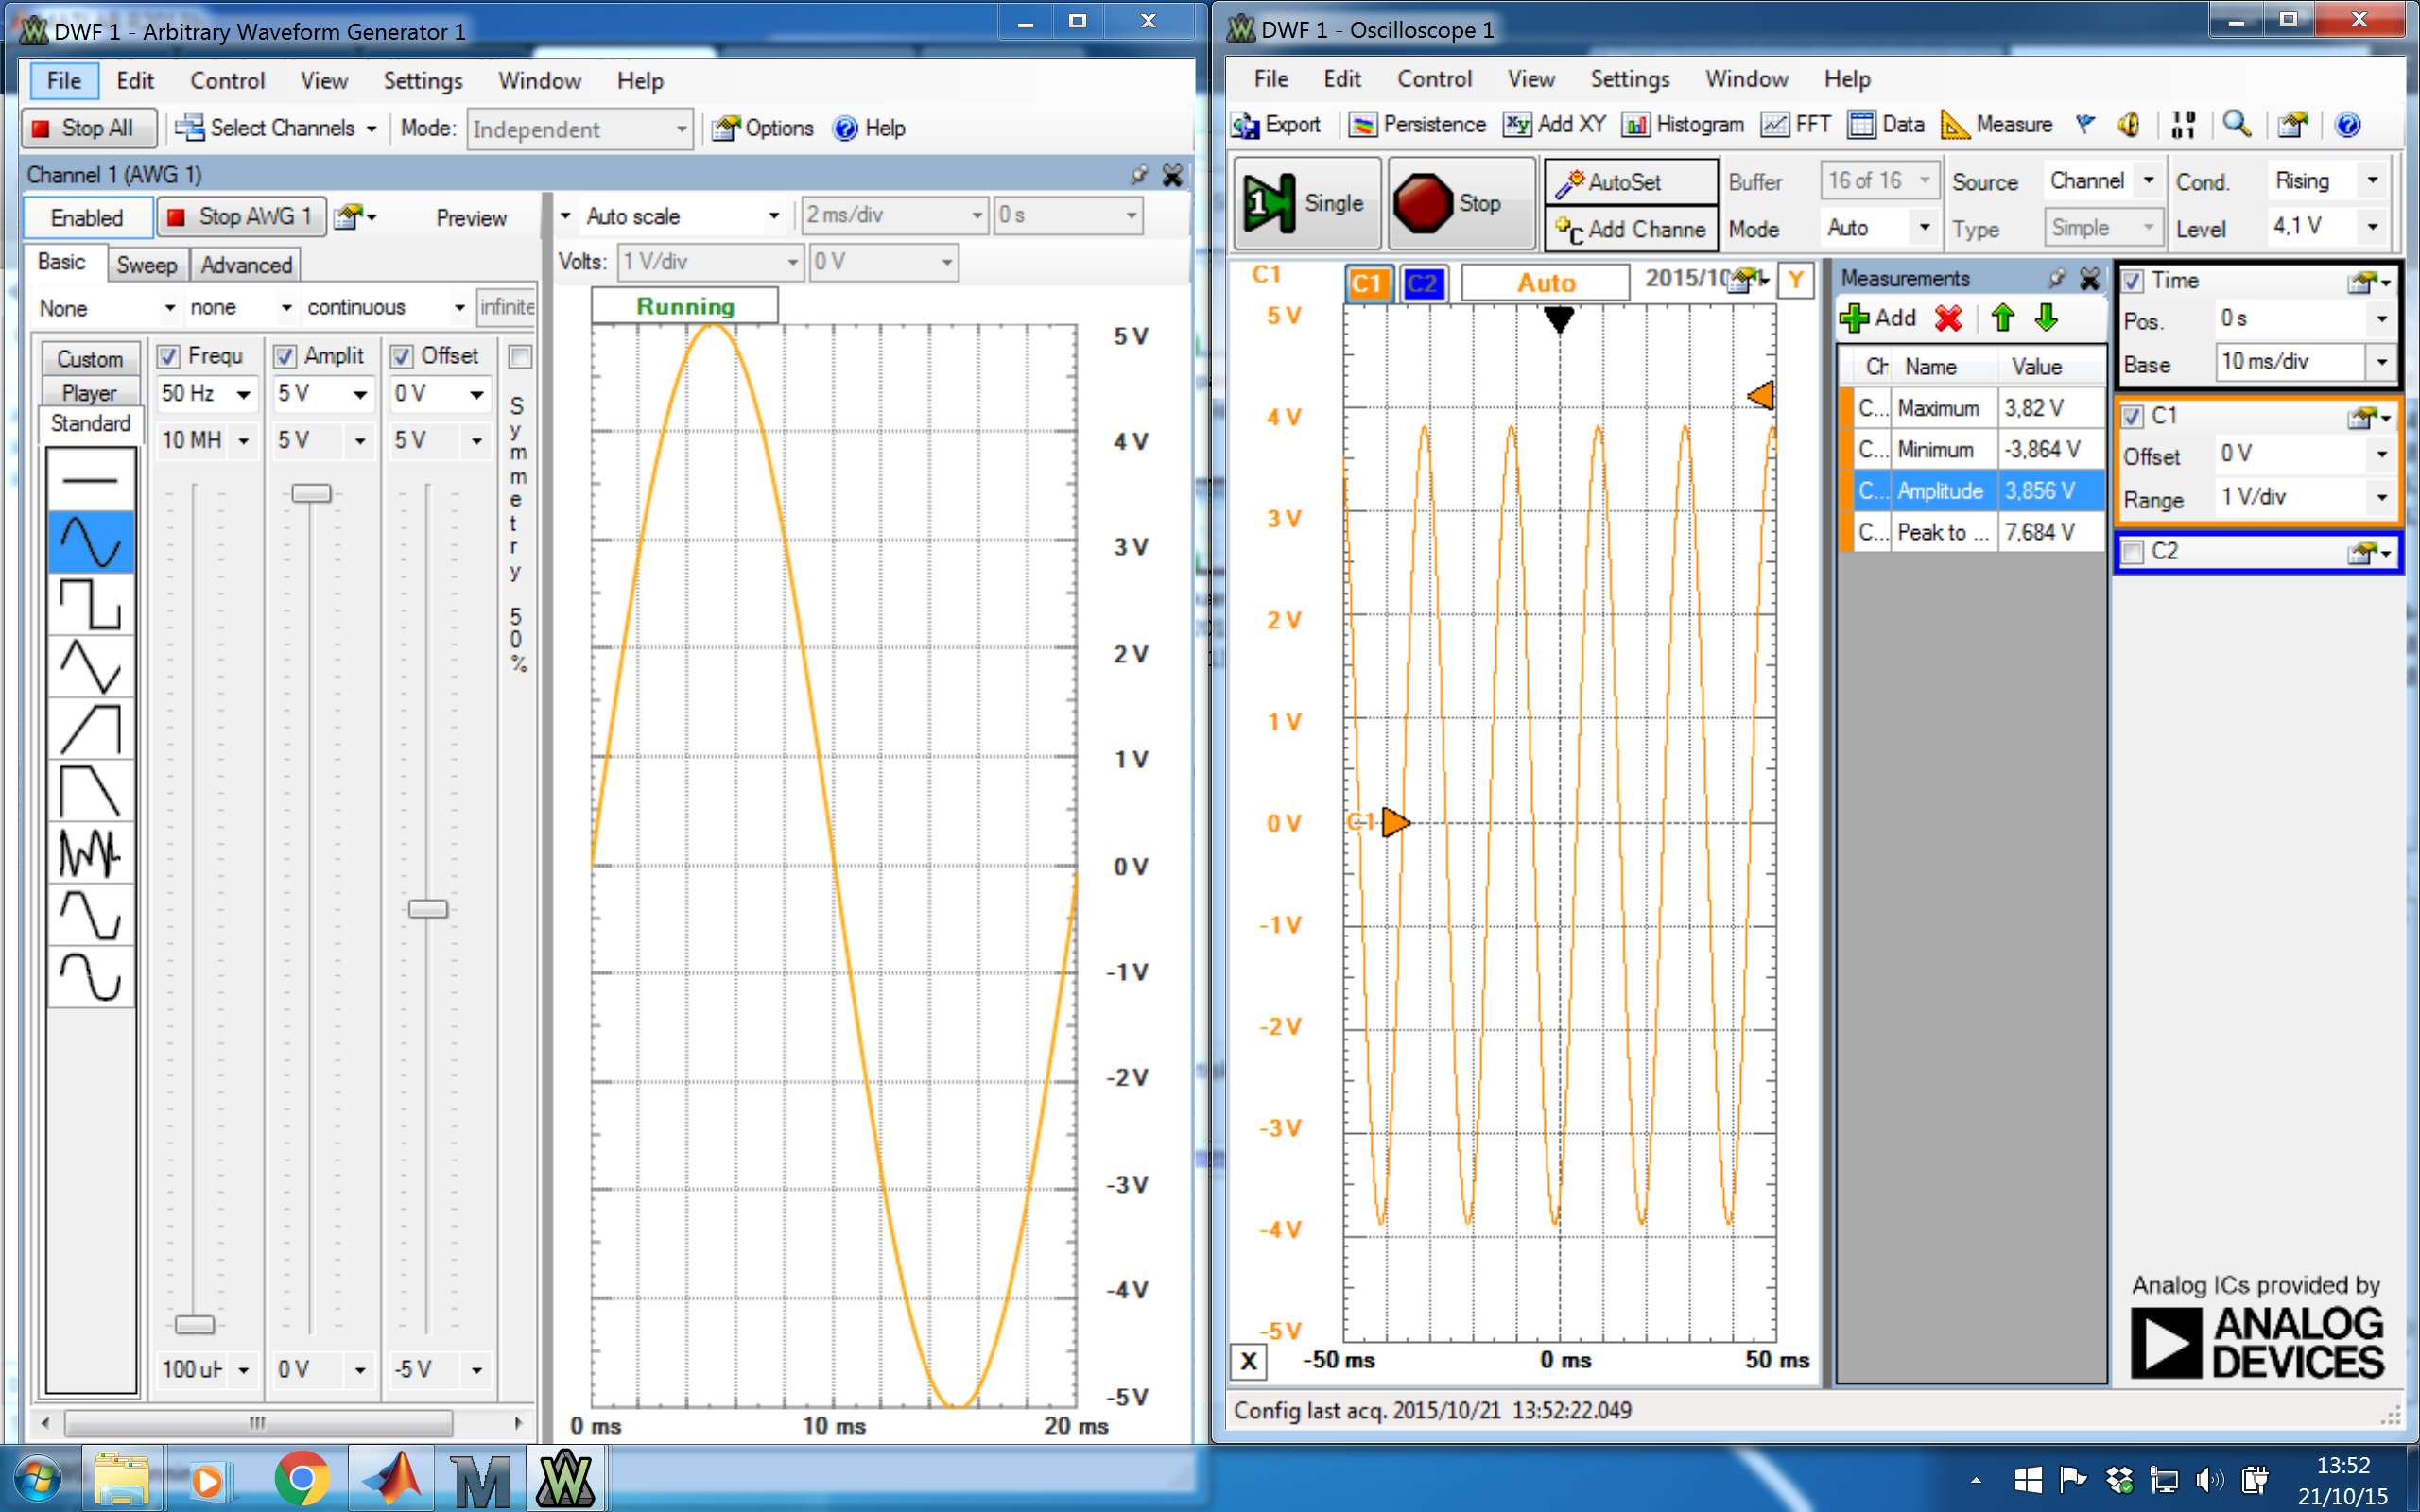
\includegraphics[width=1\textwidth]{Figurer/Lavpasfilter_Praktisk_50Hz}
	\caption{Lavpasfilter respons 50 Hz}
	\label{fig:Filter}
\end{figure}

\begin{figure}[H]
	\centering
	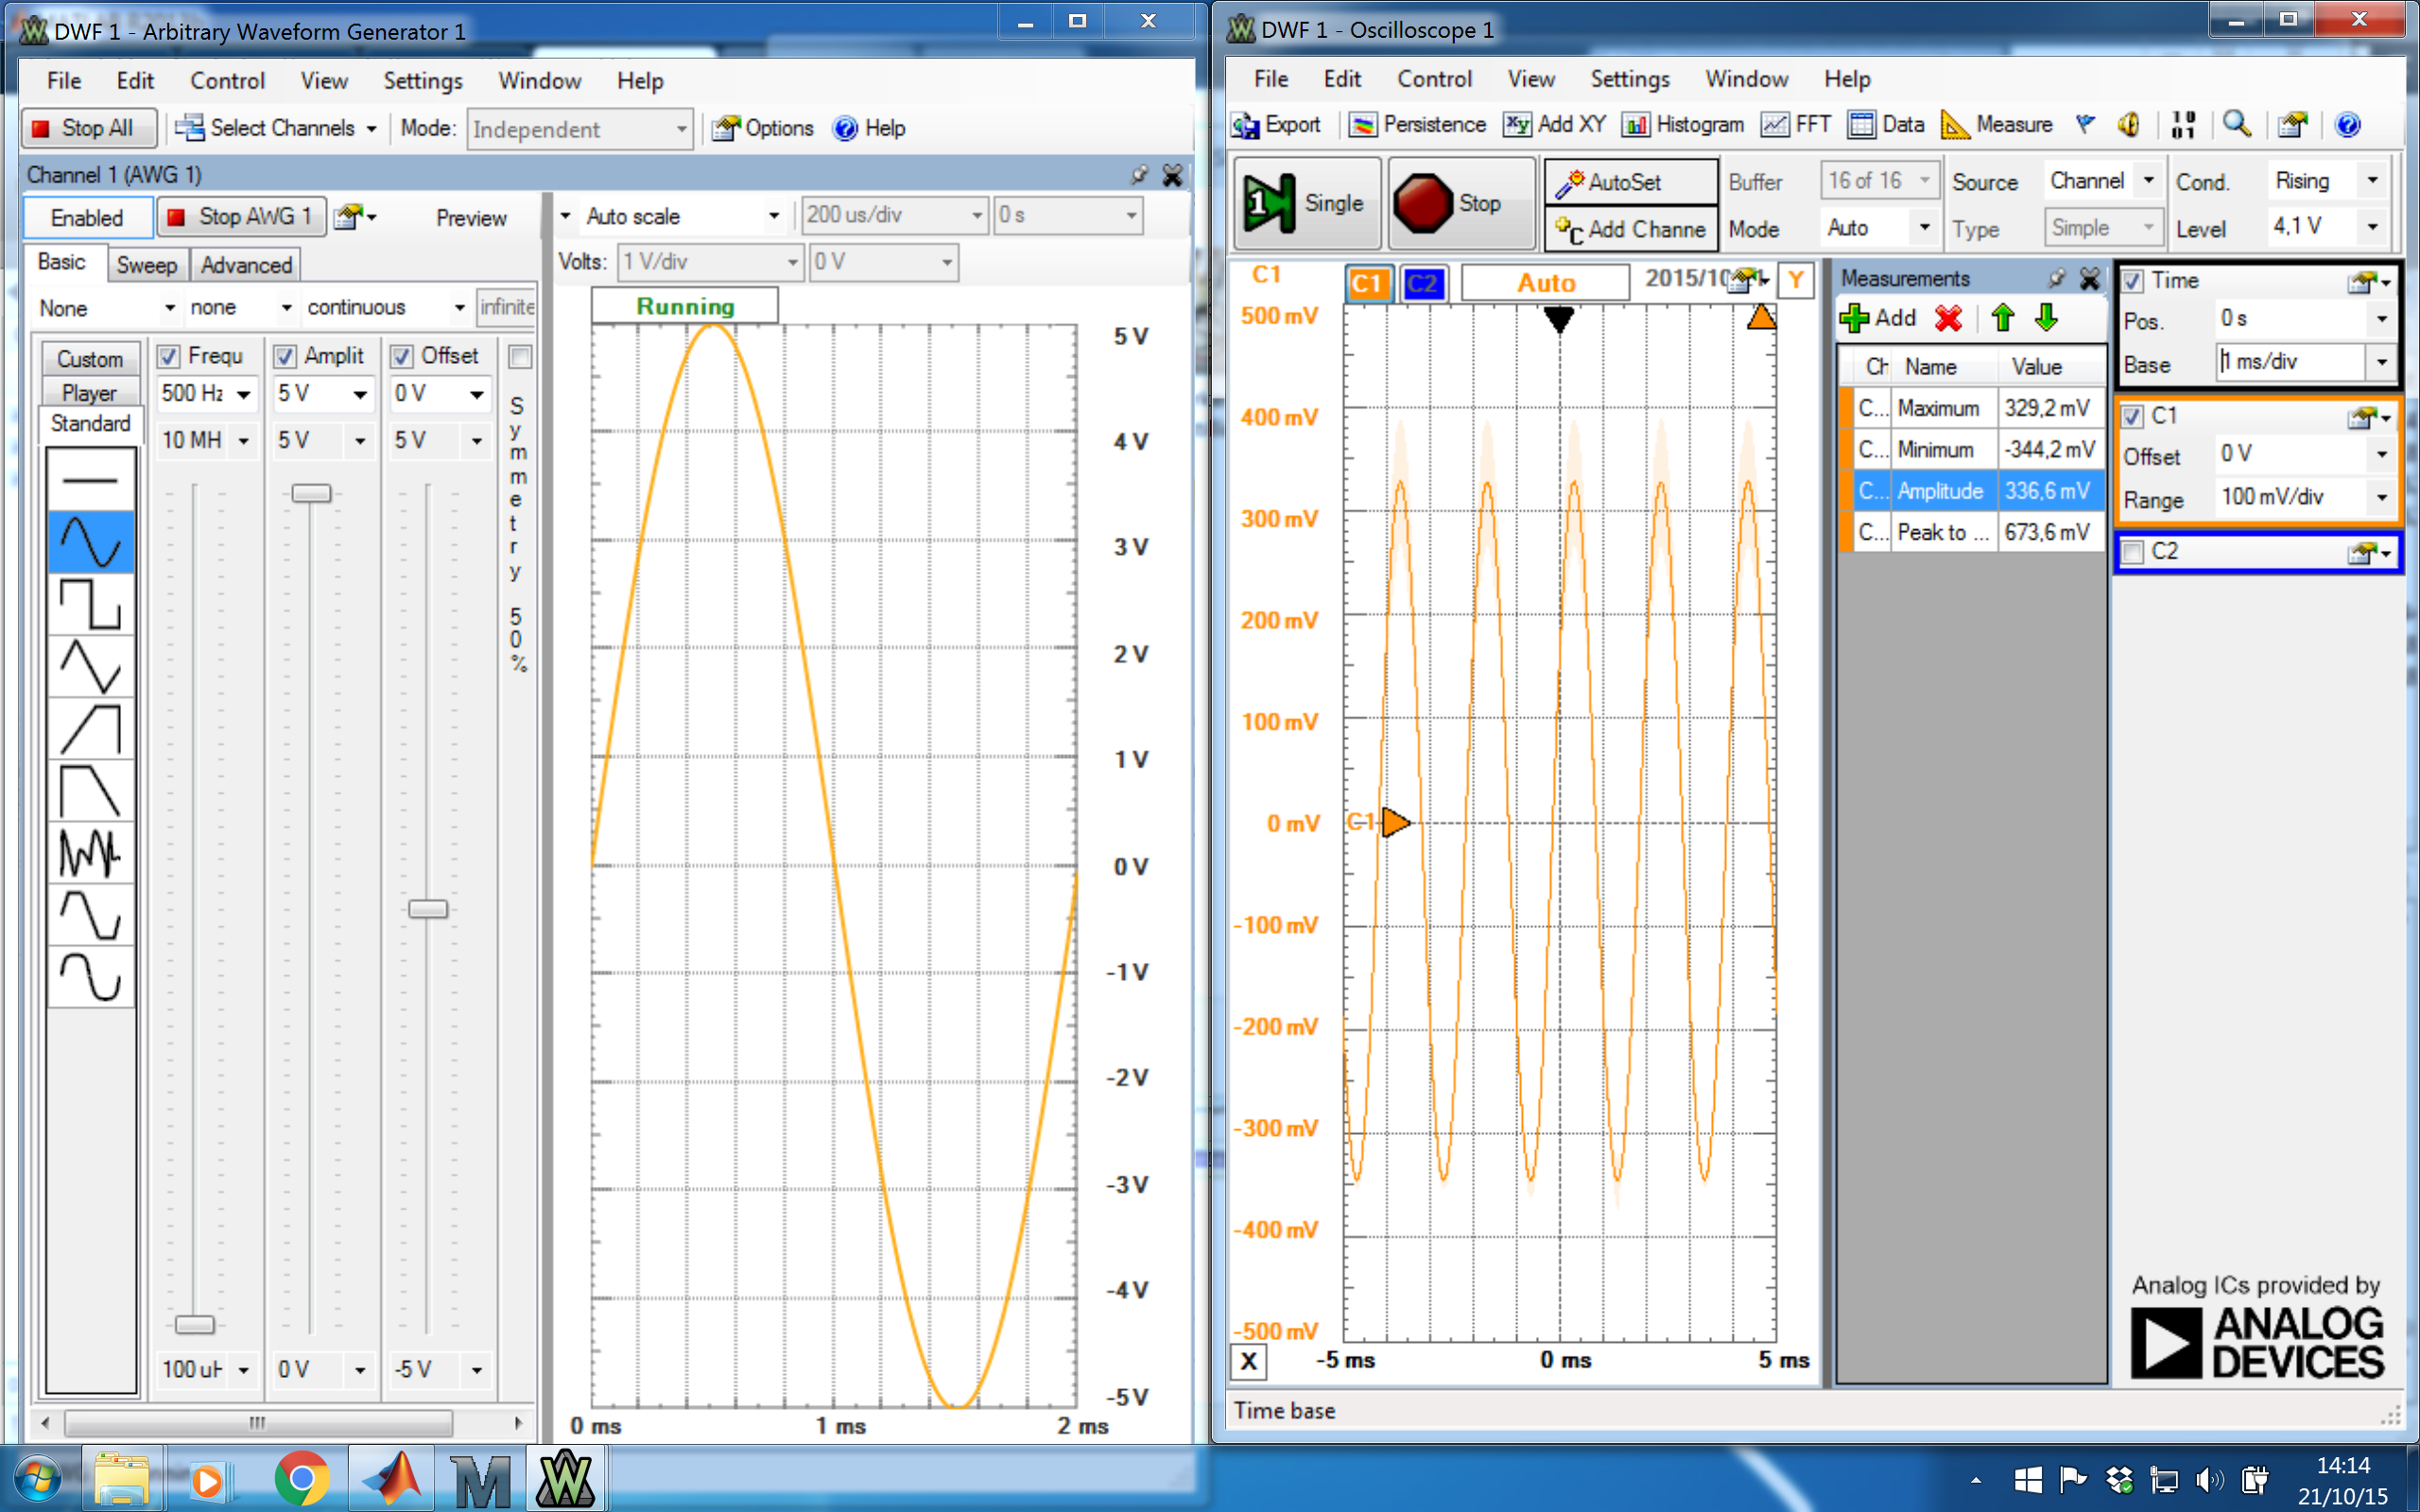
\includegraphics[width=1\textwidth]{Figurer/Lavpasfilter_Praktisk_500Hz}
	\caption{Lavpasfilter respons 500 Hz}
	\label{fig:Filter}
\end{figure}


